\graphicspath{{content/11-reference/images/}}

\chapter{Référence}

\section{Utilisation de Rsnap}

%\subsection{Créer une mission}
\begin{figure}
  \begin{center}
    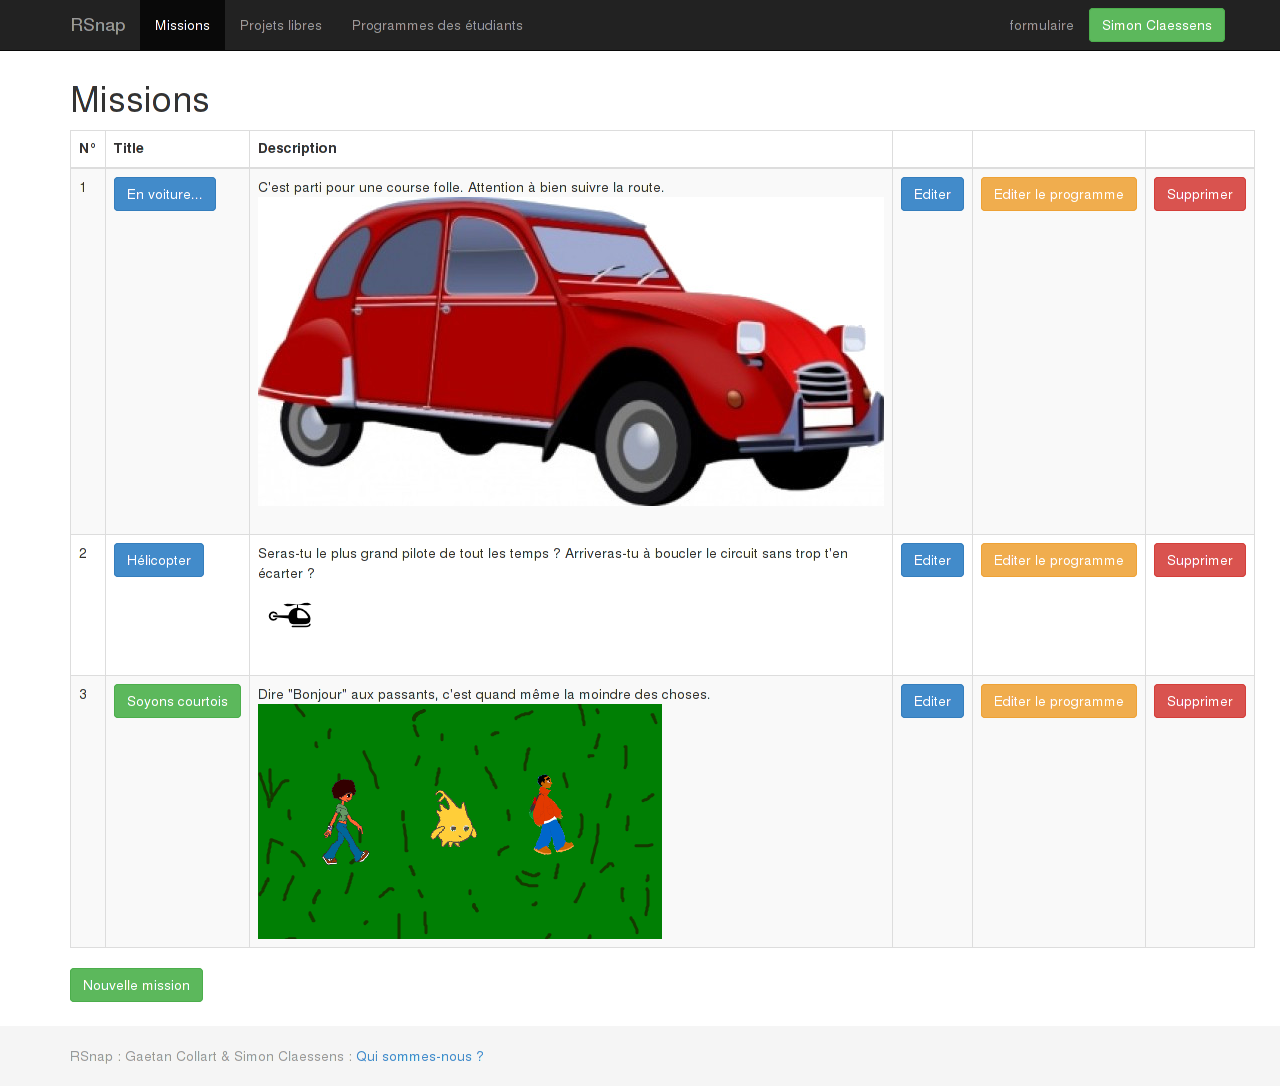
\includegraphics[width=\textwidth]{creer-mission-1}
    \caption{Page des missions}
    \label{fig:creer-mission-1}
  \end{center}
\end{figure}
\begin{figure}
  \begin{center}
    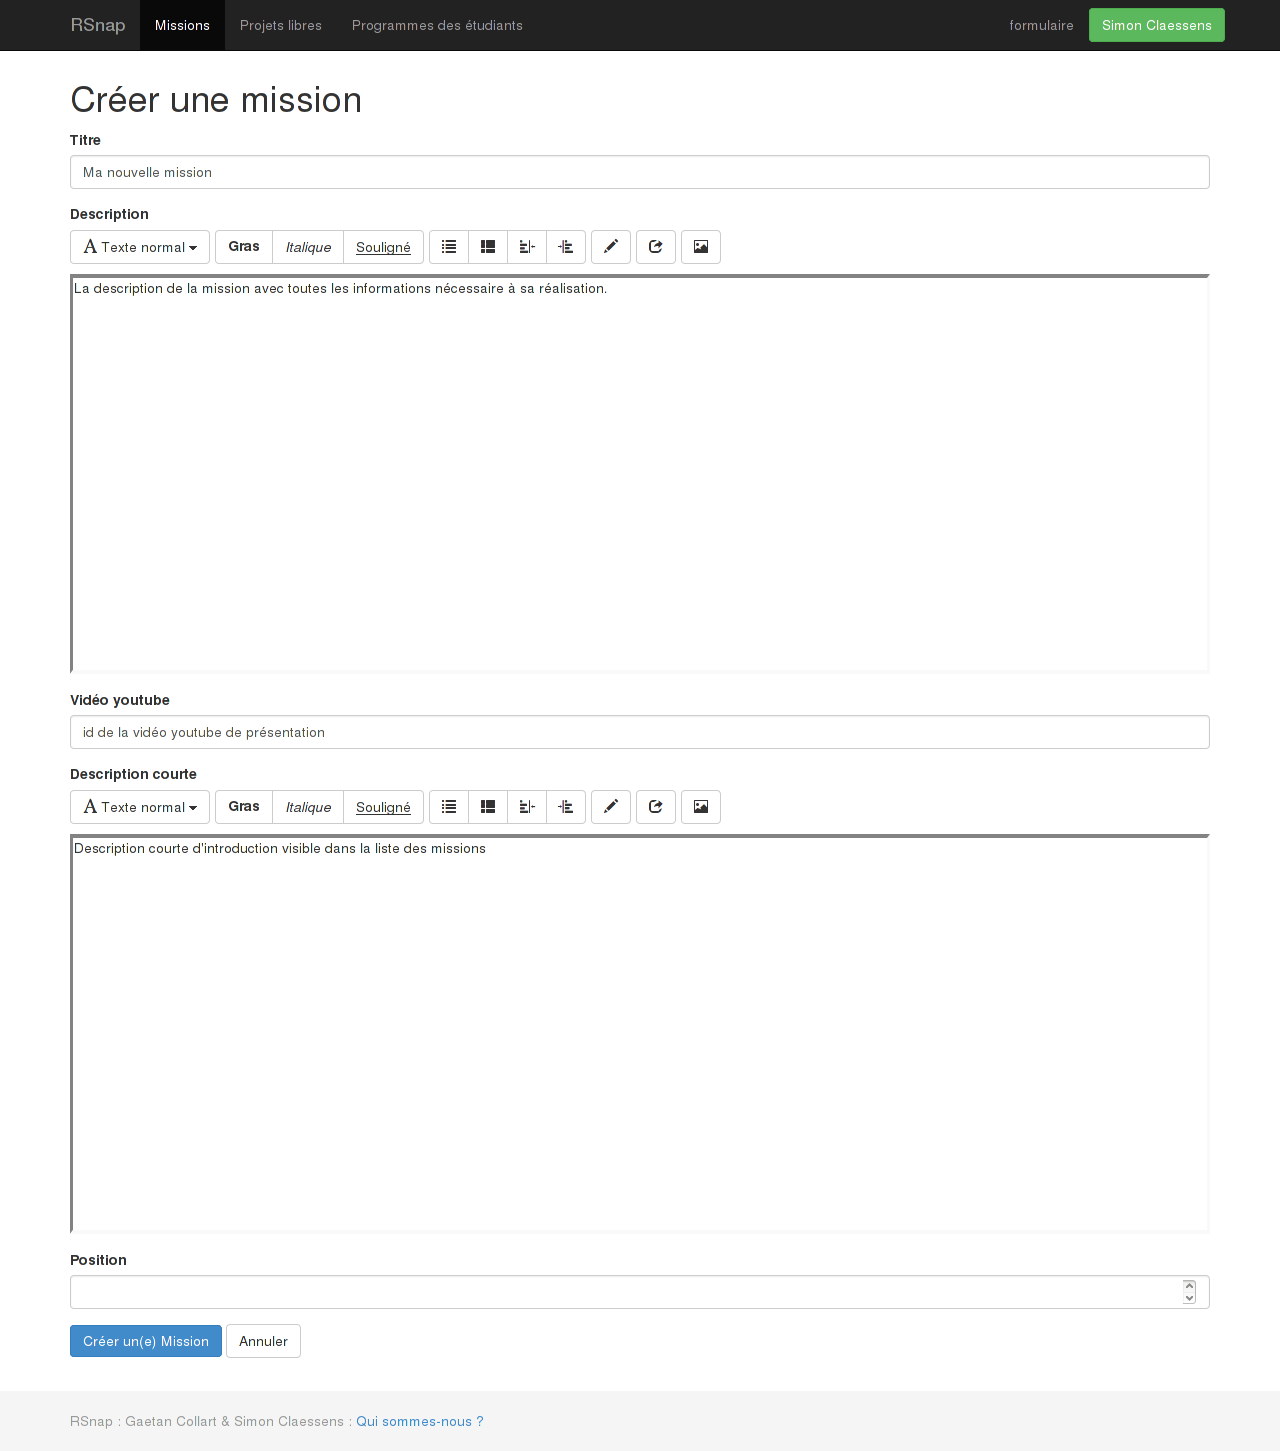
\includegraphics[width=\textwidth]{creer-mission-2}
    \caption{Création des informations de la mission}
    \label{fig:creer-mission-2}
  \end{center}
\end{figure}
\begin{figure}
  \begin{center}
    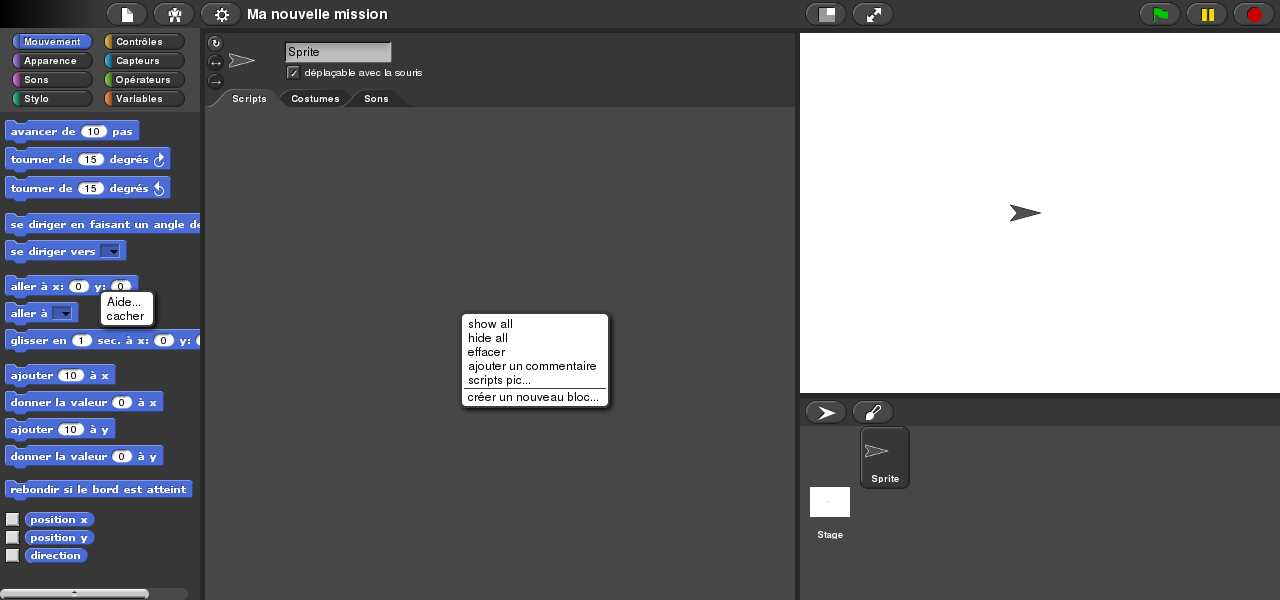
\includegraphics[width=\textwidth]{creer-mission-3}
    \caption{Création du programme de la mission}
    \label{fig:creer-mission-3}
  \end{center}
\end{figure}

%\subsection{Ordonner les missions}
\begin{figure}
  \begin{center}
    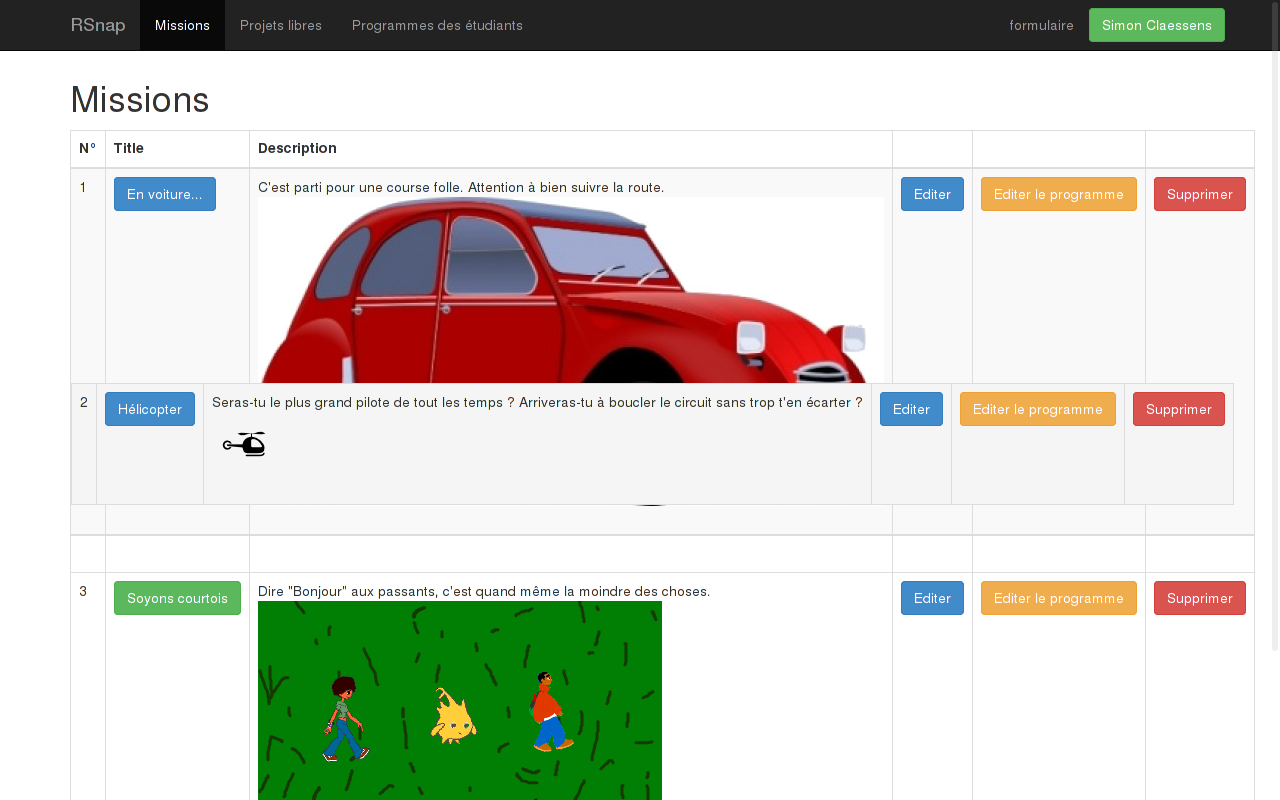
\includegraphics[width=\textwidth]{mission-order}
    \caption{Ordonner les missions}
    \label{fig:mission-order}
  \end{center}
\end{figure}

%\subsection{Corriger une mission}
\begin{figure}
  \begin{center}
    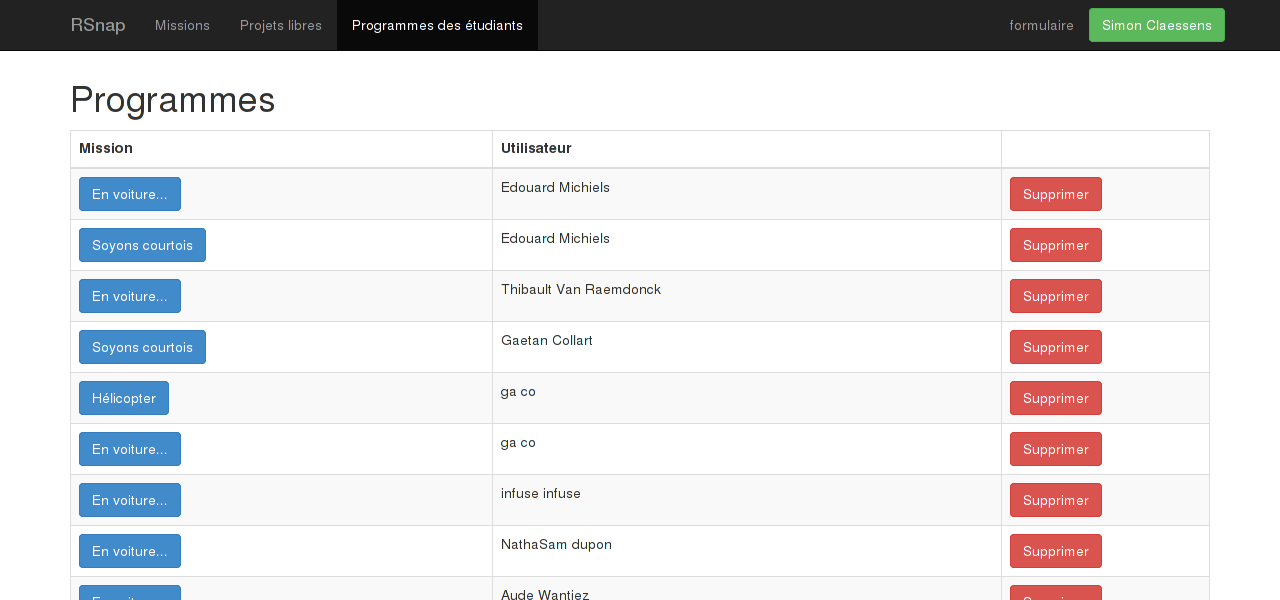
\includegraphics[width=\textwidth]{corriger-prog-1}
    \caption{Page des programmes des étudiants}
    \label{fig:corriger-prog-1}
  \end{center}
\end{figure}
\begin{figure}
  \begin{center}
    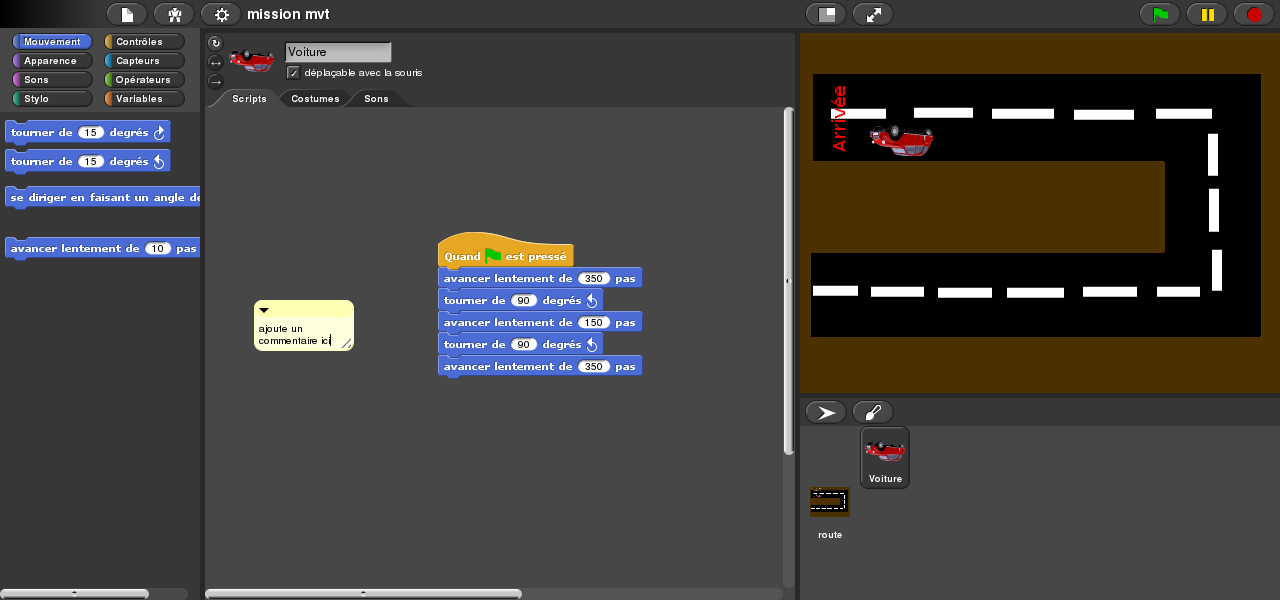
\includegraphics[width=\textwidth]{corriger-prog-2}
    \caption{Correction du programme}
    \label{fig:corriger-prog-2}
  \end{center}
\end{figure}

%\subsection{Réaliser une mission}
\begin{figure}
  \begin{center}
    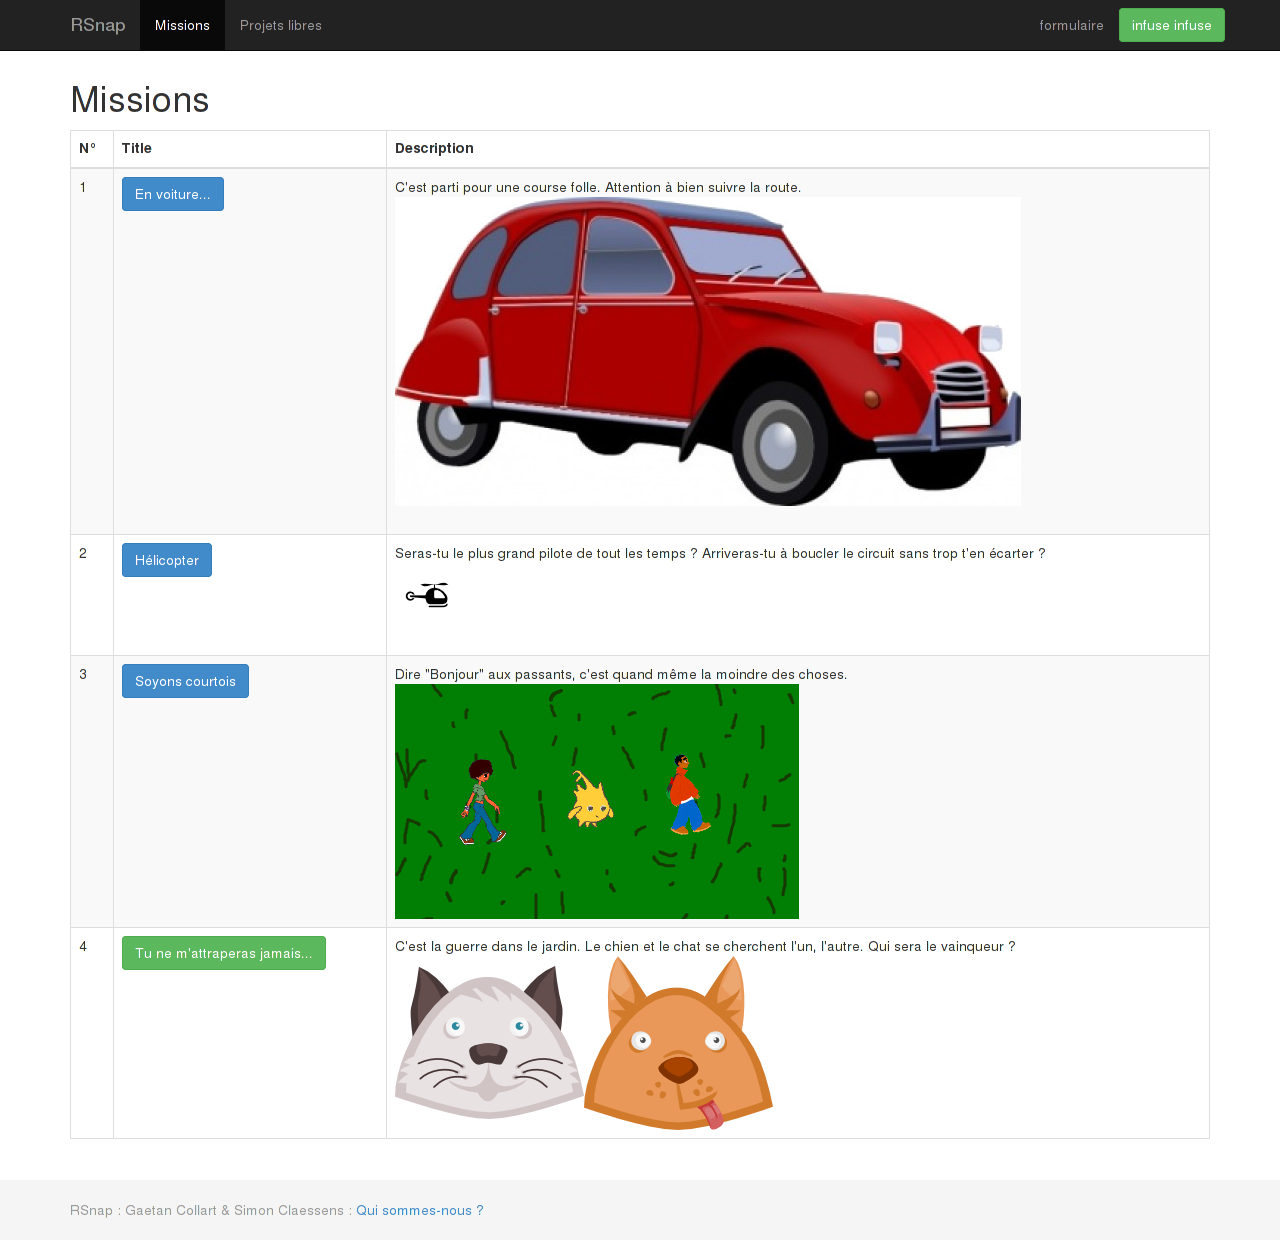
\includegraphics[width=\textwidth]{realiser-mission-1}
    \caption{Page des missions}
    \label{fig:realiser-mission-1}
  \end{center}
\end{figure}
\begin{figure}
  \begin{center}
    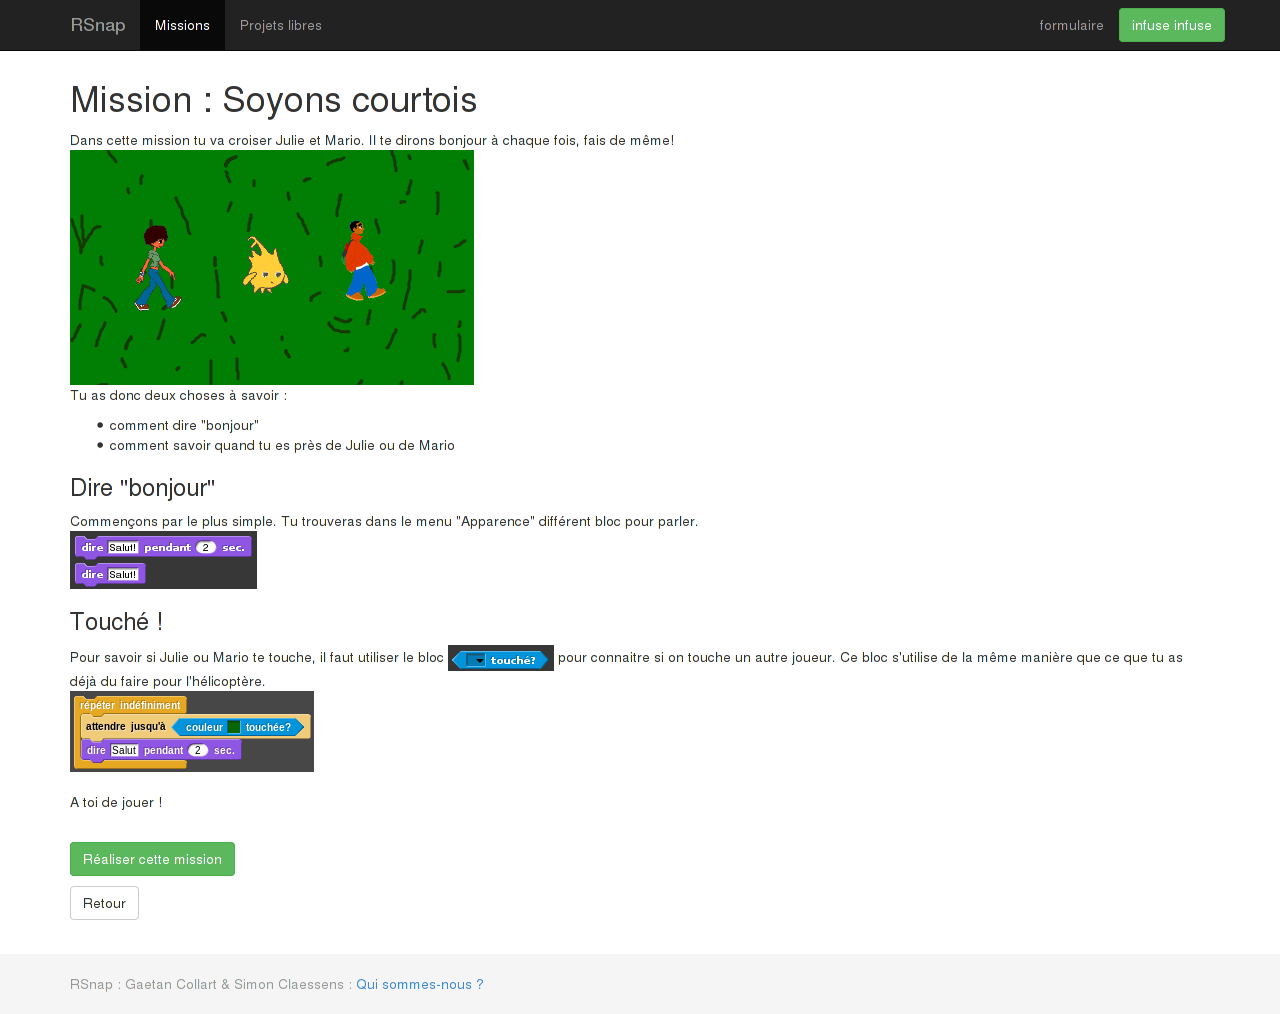
\includegraphics[width=\textwidth]{realiser-mission-2}
    \caption{Description de la mission}
    \label{fig:realiser-mission-2}
  \end{center}
\end{figure}
\begin{figure}
  \begin{center}
    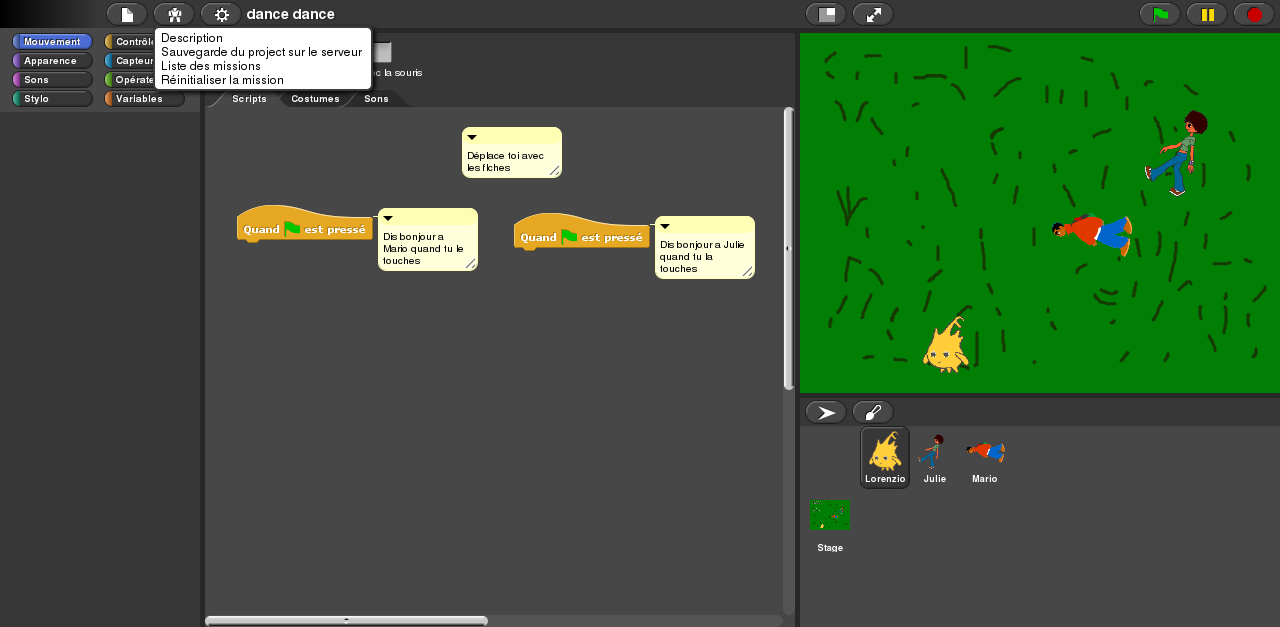
\includegraphics[width=\textwidth]{realiser-mission-3}
    \caption{Réalisation de la mission}
    \label{fig:realiser-mission-3}
  \end{center}
\end{figure}

%\subsection{Réaliser un projet libre}
\begin{figure}
  \begin{center}
    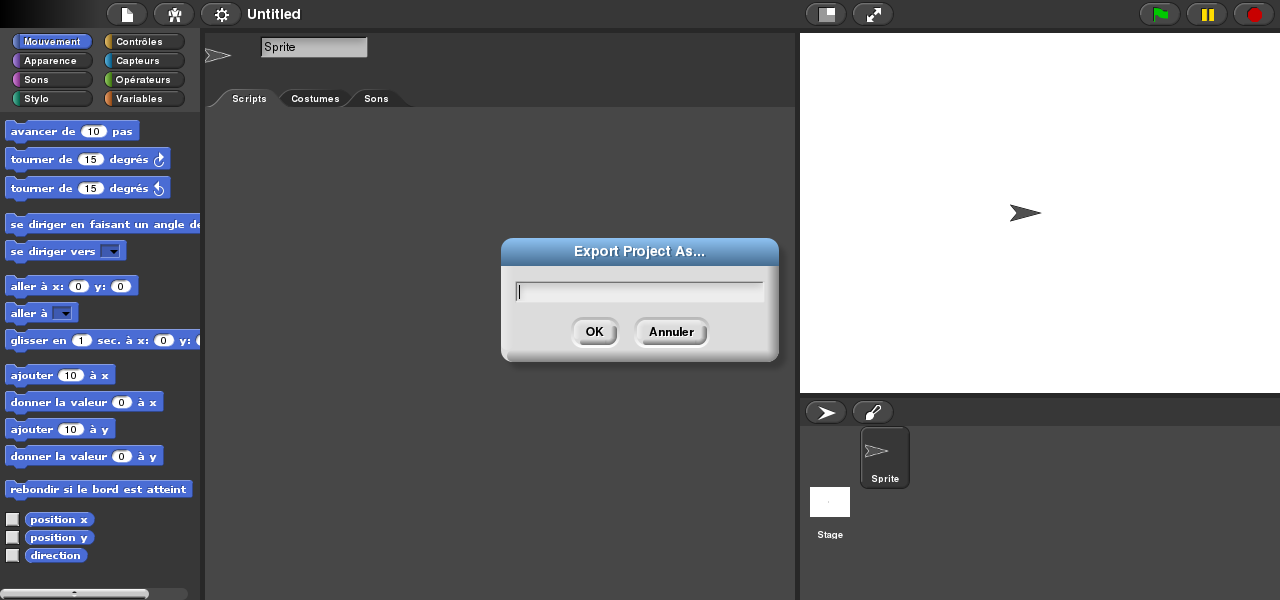
\includegraphics[width=\textwidth]{projet-1}
    \caption{Page des projets libres}
    \label{fig:projet-1}
  \end{center}
\end{figure}
\begin{figure}
  \begin{center}
    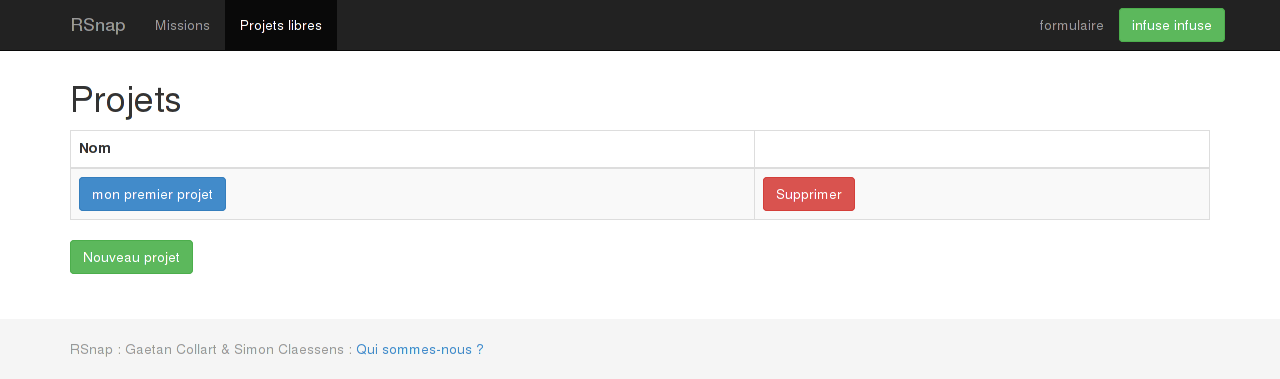
\includegraphics[width=\textwidth]{projet-2}
    \caption{Créeation du programme du projet libre}
    \label{fig:projet-2}
  \end{center}
\end{figure}

\section{Réponses du formulaire}
\begin{table}
  \caption{Réponse aux questions d'ordre général}
  \label{tab:form-perso}

  \begin{center}
    \begin{tabular}{|l|l|l|l|l|l|l|}
\hline
Je suis à ...&Je suis en ...&Je savais utiliser un ordinateur avant de venir ?&Je sais mieux utiliser un ordinateur maintenant ?&Je savais ce qu'était la programmation \\ \hline avant de venir ?&Je comprend mieux ce qu'est la programmation maintenant ?&J'ai encore des choses à vous dire.\\
Collège Cardinal Mercier&1e secondaire&3&3&4&3&\\
Collège Saint Joseph &1e secondaire&3&4&2&4&\\
Collège Saint-Joseph Chimay&1e secondaire&3&1&3&3&nan\\
college st joseph chimay&1e secondaire&2&2&1&3&\\
au college saint josephe de chimay&1e secondaire&4&4&1&4&\\
college saint joseph&1e secondaire&2&3&1&3&\\
collège saint joseph à chimay&1e secondaire&3&3&1&4&bon courrage pour votre fin d'année!!! félicitation\\
collège st Joseph chimay&1e secondaire&2&3&2&3&\\
Saint Joseph Chimay&1e secondaire&3&3&1&4&\\
Collège St Joseph  &1e secondaire&2&3&1&3&c etais cool\\
Collège St Joseph  &1e secondaire&4&4&0&0&\\
collège saint joseph&1e secondaire&4&1&1&3&amusant, des missions plus faciles que les autres, beaucoup de réfléxions.\\
college saint joseph&1e secondaire&4&1&2&4&\\
st-joseph&1e secondaire&4&4&1&4&c'etais trop cool on ces bien amuser merci !!!!!!!!!!!\\
Collège Saint Joseph &1e secondaire&4&1&4&1&\\
college saint joseph 1c8&1e secondaire&4&3&2&4&non\\
Chimay&1e secondaire&3&2&1&2&que c'était en partit quand même bien malgré le soucis\\
collège saint joseph à chimay&1e secondaire&2&2&1&4&\\
collège st Joseph chimay&1e secondaire&4&1&2&3&\\
au college saint josephe de chimay&1e secondaire&2&1&1&1&\\
st marie &6e primaire&4&4&0&4&\\
ecole st marie bousval&6e primaire&3&3&1&4&un peu plus de mission dans ce genre et des mission un peu plus compliquer pour les plus grand et des plus facile pour les plus petit\\
sainte marie&6e primaire&4&1&3&3&\\
rendeux&6e primaire&2&2&2&3&\\
ecole Ste Marie&6e primaire&4&1&1&4&PLUS VITE CET BIIIIIIIIIIIIP D'ORDINATEUR!!!!!!!!!!!!!!!!!!!!!!!!!!!!!!!!!!!!!!!!!!!!!!!!!!!!!!!!!!!!!!!!!!!!!!!!!!!\\
Sainte-Marie&6e primaire&4&2&3&4&non juste les bug\\
école St-Marie&6e primaire&4&4&1&3&\\
Ecole Sainte Marie&6e primaire&2&4&1&3&s etais trop COOL et on sais bien amusé\\
Collège du Biéreau&6e primaire&4&1&4&4&\\
aro&6e primaire&3&2&1&3&\\
aro&6e primaire&4&4&1&4&\\
aro&6e primaire&4&1&0&4&\\
 aro paul delvaux ottignies&6e primaire&2&3&1&1&c est trop dur mais sava\\
 A.R.O.&6e primaire&4&1&3&4&\\
ARO&6e primaire&4&2&3&3&\\
athenée royal paul delvaux d'ottignies&6e primaire&4&1&2&4&\\
    \end{tabular}
  \end{center}
\end{table}

